\subsection{La reprise d'antériorité}

Revenir sur les premières réflexions sur le traitement documentaire entamé par les cinémathécaires semble nous éloigner quelque peu du dépôt légal. Pourtant, les notices issues de ces premières réflexions ont pour leur majorité disparues, et ce à cause de la « reprise d’antériorité », entamée par le dépôt légal. La reprise d’antériorité consiste, pour des documentalistes, à reprendre d’anciennes notices. A ne pas confondre avec la saisie des notices cartonnées dans les nouvelles bases de données informatiques dans les années 90. Ces saisies étaient effectué par des prestataires et vérifiés par les documentalistes qui préparaient ces fiches et complétaient les informations manquantes sur les journalistes ou le matériel\footnote{(Voir entretien d'une documentaliste sur la présentation de son parcours à l'INA ~\ref{ann:transcriptions},\nameref{ann:transcriptions}), p.~\pageref{ann:transcriptions}.}. Les reprises d'antériorité, quant à elles, concernent des notices sélectionnées selon des critères patrimoniaux. Par exemple, si certaines émissions suscitent un intérêt nouveau au regard de nos modes de pensées contemporains. Elles peuvent également faire l’objet d’une reprise pour des raisons commerciales, dans le cadre d’une commande. Ces anciennes notices ne présentent plus les informations susceptibles d’intéresser les publics actuels de l’INA, mais cela ne signifie pas que l’émission décrite n’est pas digne d’intérêt, seulement que les informations susceptibles d'intéresser le public ne sont pas mises en avant. Ces émissions étaient réalisées au cours de prises d’antenne\footcite[][185]{tible2023}, en conséquent, il est difficile d’envisager que toutes les informations aient été saisies. A cela s’ajoute les erreurs humaines possibles : faute de frappe, omission volontaire ou involontaire etc. Lors d’un entretien réalisé avec une documentaliste de l’INA\footnote{(Voir entretien d'une documentaliste de l'INA sur l'impact de la politique documentaire sur les données de description ~\ref{ann:transcriptions},\nameref{ann:transcriptions}), p.~\pageref{ann:transcriptions}.}, elle évoque ainsi l’émission \enquote{Aujourd'hui madame}, qui suscita un regain d’intérêt auprès des décideurs de l’INA grâce au sujet de société qu’elle abordait qui pouvaient trouver un intérêt historique ou sociologique. Grâce à cette reprise d’antériorité on peut remettre en avant des sujets absents, des notices pour diverses raisons, pouvant être des omissions par manque de temps ou pas l’absence d’intérêt qu’ils suscitait à cette époque. Elle cite dans ce cas des propos pédophiles, n’ayant visiblement pas suscité assez d’intérêt pour être signalé dans la notice d’origine mais qui aujourd’hui peuvent intéresser toute personne effectuant des recherches dans les bases de données de l’INA. Dans un registre moins délicat, elle cite également l'émission \enquote{Pile ou Face}, une émission jeunesse qui n'avait pas été particulièrement relevée à son époque mais qui de nos jours présente un intérêt car il présente des métiers n'existant plus aujourd'hui. Malgré tout, ces reprises d'antériorité manifestent d'un choix, d'une sélection des programmes pouvant faire l'objet de reprises. Ce qui sous-entend que certains programmes ne font pas l’objet de reprises. Ainsi ils peuvent peiner à ressortir lors d’une recherche. Pour exemple, cette notice, répondant au titre d'« Images de Turquie » décrivant une actualité sur le séisme de Varto en 1966 mais n’utilisant jamais le terme « séisme ». Lors de la création de cette notice physique, elle était probablement classée dans un tiroir « catastrophe » et ou un tiroir « Turquie »\footnote{Exemple issu d’un échange de mail avec la documentaliste interrogée à la suite de notre entretien.} mais de nos jours, cette notice ne ressortira jamais pour une personne effectuant des recherches sur le séisme de Varto ou encore sur des catastrophes naturelles en Turquie. 

\begin{figure}[H]
	\centering
	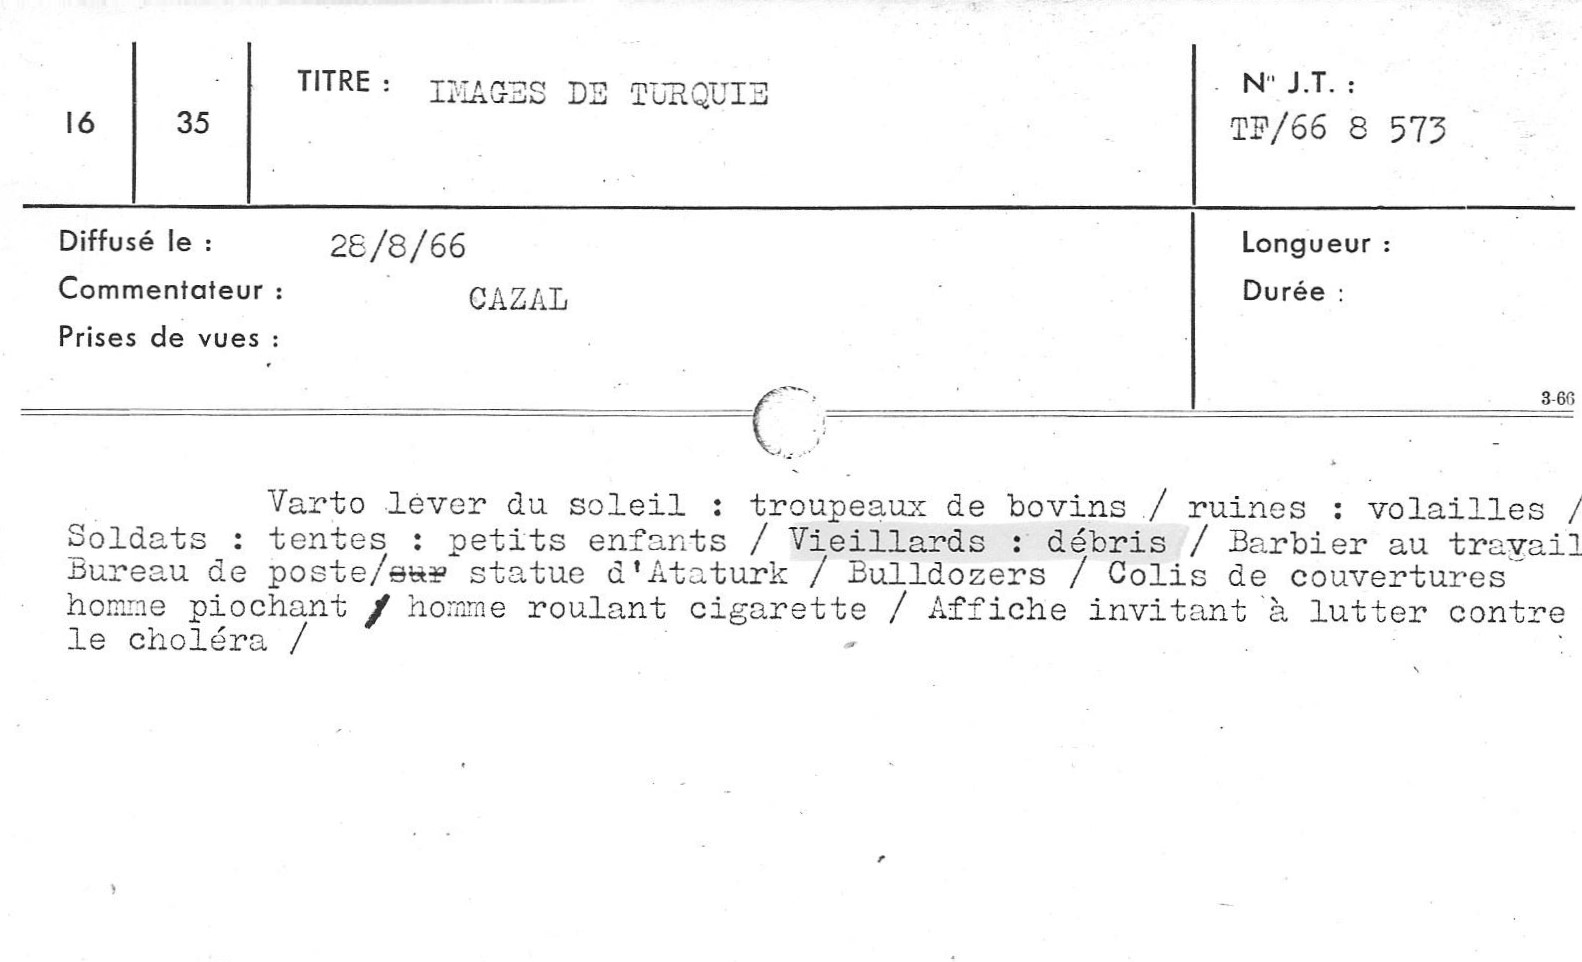
\includegraphics[width=1\linewidth]{./illustrations/notice_turquie_papier.jpg}
	\caption{Photocopie de la notice physique de la notice \enquote{Images de Turquie}}
	\label{fig:imgturquie}
\end{figure}

Pour finir, nous pouvons souligner que ces fiches ayant fait l'objet d'une reprise d'antériorité écrasent les fiches précédentes. L’indexation utilisée pourraient pourtant trouver une valeur aujourd'hui et contribuer à définir une cartographie des traitements documentaires. Au contraire, dans notre cas, elle la complexifie car cette destruction n'est pas systématique à chaque période non plus. Les fiches papiers datant d'avant 1975 ont été conservées par l'INA, certaines sont conservées dans les locaux de l'INA à Bry-sur-Marne, d'autres au centre de conservation de l'INA à Saint-Remy-l'Honoré. Les fiches papiers crées après 1975 ont elles été détruites et la seule trace de leur existante figure dans le champs \enquote{notes} de la notice, indiquant que cette notice a été reprise à telle année\footnote{(Voir entretien d'une documentaliste de l'INA sur l'impact de la politique documentaire sur les données de description ~\ref{ann:transcriptions},\nameref{ann:transcriptions}), p.~\pageref{ann:transcriptions}.}.

\begin{figure}[H]
	\centering
	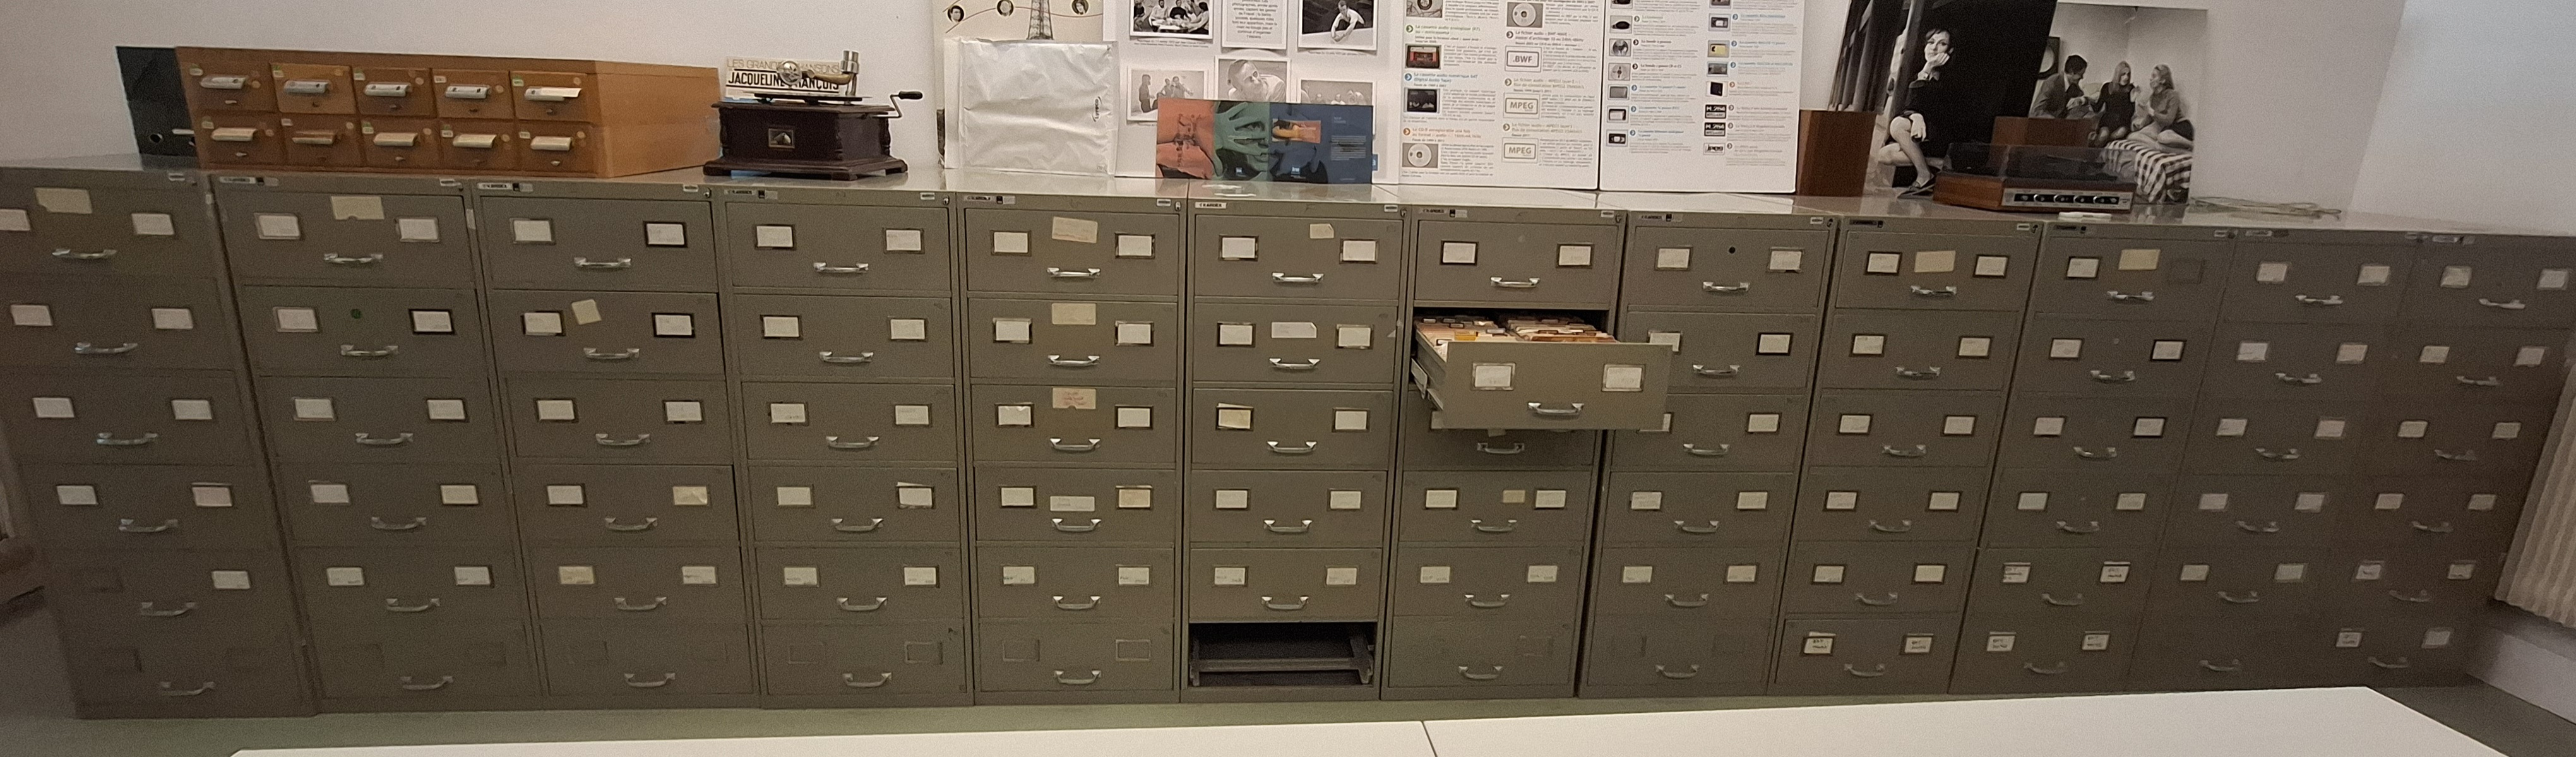
\includegraphics[width=1\linewidth]{./illustrations/tiroir_bry.jpg}
	\caption{Tiroir de classement de fiche papier conservés à Bry 1}
	\label{fig:imgtiroirbry}
\end{figure}

Nous soulevons ainsi un premier obstacle à la compréhension des bases de données. Des notices correspondant à au minimum deux politiques documentaires cohabitent, une politique commerciale et une politique patrimoniale. Les campagnes de reprises d'antériorité sont nombreuses et peu documentées. De plus, certaines notices, considérées lacunaires sont parfois reprises par des documentalistes au cas par cas, parfois sur le signalement de professionnels de l'audiovisuel via la plateforme inamediapro.fr\footnote{(Voir entretien de Pascal Lebeurier sur les outils et services de l'INA ~\ref{ann:transcriptions},\nameref{ann:transcriptions}), p.~\pageref{ann:transcriptions}.}, ce qui diminue une fois de plus le lisibilité des collections dans les bases de données. 

En abordant la reprise d'antériorité comme première approche de la politique documentaire qu'apporte le dépôt légal, nous pouvons souligner l'importance que prend le choix. Un nouveau regard se pose sur les contenus qu'ils conservent et l'usage dont on pourrait en faire. On questionne ce que les publics attendent, les informations qui pourraient les intéresser. Bien que ces reprises concernent également les archives professionnelles, la politique documentaire doit désormais convenir à d'autres publics, différent de ceux qui ont produit ces fiches. L'éloignement temporel que l'institution prend avec ses première notices de description et l'instauration du dépôt légal donnent une place importante à la patrimonialisation de leurs documents. Il n'est plus question de les conserver pour être réutilisé dans un temps court par un public qui connaît ces collections et sa description mais bien pour être communiqué, sur le temps long, autant à un public externe qu'à un public interne n'ayant pas conçu ces descriptions. L'importance du choix dans ces politiques consiste donc à déterminer, à prévoir les informations que l'on souhaitera voir ressortir. Cette notion est particulièrement importante quand on considère que le périmètre du dépôt légal s'étend, accentuant l'importance du choix des contenus à décrire et des informations à inscrire sur ces fiches. 

\subsection{Les types de traitements documentaire}

Il n’est plus question de sélectionner les informations que l’on écrit dans les notices selon le temps dont on dispose mais de sélectionner parmi une grande quantité de données, quelles émissions méritent d’avoir une notice plus fournie qu’une autre. Auparavant, il est essentiel de rationaliser, les 28 millions d’heures captées au titre du dépôt légal évoquées plus tôt. Parmi elles, une partie outrepassent les obligations du dépôt légal mais pour mieux comprendre quelles émissions sont comprises dans le cadre du dépôt légal, il faut revenir à ses tout débuts, avant que les avancées technologiques ne permettent de capter une centaine de chaînes 24 heures sur 24. A ses débuts, le dépôt légal était un \enquote{dépôt} au premier sens du terme et c’était aux chaînes de télévision de déposer leurs émissions, qui étaient ensuite décrites par les documentalistes. Les émissions déposées étaient les émissions de production française diffusées pour la première fois. Ces émissions étaient et sont toujours les émissions décrites. Aujourd’hui, toutes les heures de diffusions captées au titre du dépôt légal sont conservées par l’INA mais seules les premières diffusions de production françaises sont décrites. Ainsi s’opère une première différence concernant les informations de descriptions des émissions. Si l’émission a été captée mais qu’elle ne répond pas à ces premiers critères pour être décrites par un ou une documentaliste, les données de descriptions dans la base de données correspondent aux imports de documentation externe à l’INA. Ils comprennent les grilles du programmes télé\footcite[Pour exemple :][]{admin} ou encore des informations sur les audiences\footcite[Pour exemple :][]{sensio}. Ces données sont rentrées, complétées et vérifiés par des TGDM, des Techniciens de gestion de données multimédia. NB : Revoir pour définition plus précise. 

La réflexion sur le traitement documentaire ne s’arrête pas là car il reste une quantité conséquente de données qui ne peuvent pas toutes êtres prises en charges. S’effectue alors une sélection des émissions sur lesquelles un traitement plus conséquent sera effectué. Loin d’être exceptionnelle, ce choix a déjà été effectué par la BNF, qui pour faire face à une quantité de données numériques massive applique par exemple un traitement moins poussé aux manuels scolaire, considérés moins pertinent pour la recherche\footcite[][70]{bermès2024}. A l’INA, le traitement documentaire est divisé en plusieurs types, identifiés par des codes. La liste qui suit les décrit, en excluant les données de description déjà présentes dans les types de traitements précédents :
\begin{itemize}
	\item \textbf{IDENT}, pour \textbf{identification} correspond à l’absence de traitement documentaire, les notices correspondant à ce traitement doivent comprendre, grâce aux imports : le titre, le générique correspondant aux personnes ayant participées à l’émission, devant ou derrière la caméra, la typologie de l’émission (Journal Télévisé, Documentaire etc\dots) et la nature de production (si l’émission est produite par la chaîne de diffusion ou non).
	\item \textbf{CATS}, pour \textbf{Catalogage signalétique} présente strictement les mêmes informations que IDENT mais vérifiées par un ou une documentaliste. C'est à partir de ce type de traitement que l'on considère que nous nous situons dans du traitement documentaire à proprement parlé car il y a l'intervention d'un ou d'une documentaliste.
	\item \textbf{CATED}, pour \textbf{Catalogage avec descripteurs}. Ce traitement ajoute les descripteurs, correspondant à des mots clés.
	\item \textbf{CATSY}, pour \textbf{catalogage synthétique}. Il ajoute un « chapeau », résumant le contenu de l’émission et le type d’images diffusées.
	\item \textbf{CATA}, pour \textbf{catalogage analytique} auquel s’ajoute un résumé dans lequel sont décrites les principales séquences et une liste des intervenants dans l’émission si il excèdent 5.
	\item \textbf{IND}, pour \textbf{Indexation de contenu} qui propose un résumé plus précis avec une description chronologique détaillée des différentes phases de l’émission, presque au plan par plan\footnote{(Pour plus de détail, consultez la fiche d'aide au dépôt légal ~\ref{ann:aidedl},\nameref{ann:aidedl}), p.~\pageref{ann:aidedl}.}.
\end{itemize}

C’est au cœur de l’utilisation de ces types de traitement que né le projet de cartographie du traitement documentaire. En effet, il n’y a pas, avant la naissance de ce projet, de récapitulatif clair et complet de la chronologie des traitements appliqués aux chaînes et aux émissions captées au titre du dépôt légal par l’INA. La sélection est faites selon les usages que l'on fera de ces images et des ressources que nécessitent leur traitement mais ces informations sont transmises par mails et ces derniers sont finalement perdus dans des boîtes mails personnelles ou supprimés. Le savoir sur la chronologie des applications de traitements repose donc en partie sur les souvenirs des documentalistes \footnote{(Voir entretien d'une documentaliste de l'INA sur l'impact de la politique documentaire sur les données de description qui évoque le traitement documentaire de \enquote{Soir 3} mais qui demande de ne pas trop d'appuyer sur ce savoir étant donné que cette information remonte au début de sa carrière ~\ref{ann:transcriptions},\nameref{ann:transcriptions}), p.~\pageref{ann:transcriptions}.}. De plus certaines considérations se perdent. Par exemple, malgré le fait que les traitements CATS sont considérés comme du traitement documentaire car cela suppose qu’un documentaliste vérifie les informations, dans les faits, le temps manque pour ces vérifications. C’est pourquoi, lors des réflexions de ce projet de cartographie du traitement documentaire, il a été décidé que les notices CATS ne seraient pas comprises dans ce que nous considérons comme du traitement documentaire\footnote{(Voir Cahier des charges du projet de cartographie du traitement documentaire ~\ref{ann:cdc},\nameref{ann:cdc}), p.~\pageref{ann:cdc}.}. Pour appuyer ces considérations, les notices de types IND sont assez rares et ont été progressivement abandonnées dans les années 90 pour des raisons d’économie de temps. Ainsi, même si une personne effectuant des recherches dans les bases de données décide de rechercher les notices IND car il recherche des descriptions très précises, au plan par plan, des émissions, il risque faire ressortir très peu de résultats. Surtout dans une temporalité plus récente, et il ne pourra pas comprendre pourquoi. Pour terminer sur ces défauts dans l'utilisation des types de traitement documentaires, certaines informations ne sont pas transmises au même moment aux documentalistes et aux TGDM, chargés de déterminer quel traitement documentaire est appliqué à une émission donnée. De cette façon, certaines émissions peuvent être indiquées d’un type de traitement en particulier mais ne pas avoir été décrit par un.e documentaliste, voire pas décrit du tout. 

Si nous ajoutons les notices précédant la mise en place du dépôt légal et de ces différents types de traitement, nous commençons à visualiser les problèmes qui s’opposent à la pleine compréhension des bases de données de l’INA pour un public extérieur autant que pour un primo-arrivant à l’INA. En prenant place à l'INA, le dépôt légal entraîne une réflexion sur le traitement documentaire, les politiques documentaires reflètent cette évolution en questionnant les informations qui doivent être renseignées en fonction de différents critères visant à mettre en avant les informations dont les chercheurs, nouveaux public de l'INA aurait besoin. Cette réflexion n'est pas la seule influence qu'a eu le dépôt légal sur le traitement documentaire. A un niveau strictement humain, l'INA divise ses services de traitement de ses collections en deux. Cela entraînera un déséquilibre dans le traitement documentaire qui plus de 30 ans après la création du dépôt légal a toujours des conséquences majeure sur l'accessibilité aux collections. 